\begin{frame}{Apporterende jagthunde}

\vspace{1em}

\begin{columns}[c] % c = center vertically

\column{0.05\textwidth} % Venstre margin

\column{0.7\textwidth} % Midten: Bullets

\small

\raggedright

\begin{itemize}

\itemsep0.6em % Justér afstand mellem bullets

\item Hovedopgaven er at \textbf{finde og bringe nedlagt vildt} til jægeren (apportere).
\item Skal være \textbf{skudfast} og have en \textbf{blød mund} for ikke at ødelægge vildtet.
\item Er nødvendig ved jagt med haglgevær på ikke-klovbærende vildt på landarealer (§ 24).
\item Er ofte velegnede \textbf{familiehunde} grundet deres samarbejdsvilje.
\item \textbf{Racer}: Labrador Retriever, Golden Retriever, Flatcoated Retriever, Chesapeake Bay Retriever.

\end{itemize}

\column{0.25\textwidth} % Højre: Ikon

\centering

\vspace{0pt}

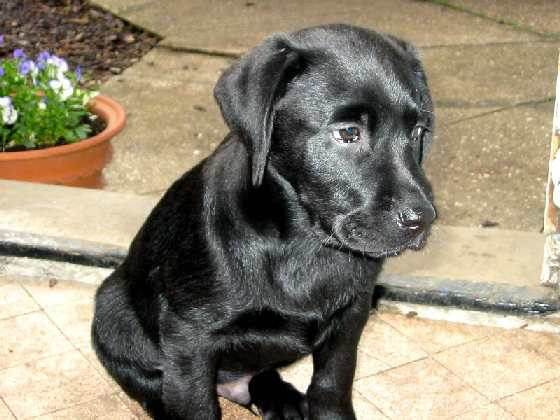
\includegraphics[width=0.9\linewidth]{Billeder/Jagthunde/apporterende/labrador.jpg} % Ikon af apporterende hund

\end{columns}

\end{frame}